% This procedure has three sub-procedures in each paragraph below.
% \begin{defn}[Loop Path]
%   \label{def:looppath}
% A simple transition path
% $\tpath \in \paths(\absG(c))$ for the program $c$, is a path on its abstract transition graph $\absG(c) = (\absV(c), \absE(c))$ with 
% \begin{itemize}
% \item a vertices sequence $(l_0, \ldots, l_n)$, where $l_i \in \absV(c)$ for every $i = 0, \ldots, n$ and
% %
% \item an edge sequence $(e_1, \ldots, e_n)$, where $e_i = (l_{i - 1}, dc_i, l_{i}) \in \absE(c)$ for every $i = 1, \ldots, n$,
% \end{itemize}
% %
% satisfying:
% \begin{itemize}
%   \item $l_i \neq l_j$ for every $i = 0, \ldots, n$ and $j = 0, \ldots, {n - 1}$,
%   \item $l_0$ is either the program point of a loop header or the program entrance ($l_0 = 0$),
%   i.e., $l_0 \in \loopl(c) \cup \{ 0 \}$
%   \item and $l_n$ is either the program point of a loop header or the program exit ($l_n = \lex$),
%   i.e., $l_0 \in \loopl(c) \cup \{ \lex \}$.
% \end{itemize}
% \end{defn}
% \subsection{Program Rewriting}

% \paragraph{The Simple Transition Path}
% We first collect the loop headers $\loopl(c) \subseteq \lvar(c)$ from a program $c$, which is the set of all program points corresponding to the loop headers in program $c$.
% \begin{defn}[Loop Headers ($\loopl : \cdom \to \mathcal{P}(\ldom)$)]
%   \label{def:loopl}
%   \[
%   \loopl(c) \triangleq 
%   \left\{
%     \begin{array}{ll}
%       \{\}  & {c} = \clabel{\assign x e}^{l} \\
%       \loopl({c_1}) \cup \loopl({{c_2}})  & {c} = {c_1};{c_2} \\
%       \loopl(c_t) \cup \loopl({{c_f}})   & {c} =\eif(\clabel{\bexpr}^{l}, c_t, c_f) \\
%   \loopl(c_w) \cup \{l\}, &  {c}   = \ewhile \clabel{\bexpr}^{l} \edo (c_w)
%   \end{array}
% \right.
% \]
%   \end{defn}
% \begin{defn}[Simple Tansition Path]
%   \label{def:tpath}
% A \emph{simple transition path}
% $\tpath \in \paths(\absG(c))$ for the program $c$, is either a simple cyclic path, which has the same start- and end-point
% or a simple path has either different while loop headers, the program entrance or exit as its start- and end-point
% without visiting any loop header inside the path.
% \\
% Specifically, a path $l_0 \xrightarrow{dc_0} l_1 \xrightarrow{dc_1} \ldots l_n \in \paths(\absG(c))$ with the
% vertices sequence $(l_0, \ldots, l_n)$, where $l_i \in \absV(c)$ for every $i = 0, \ldots, n$ and
% %
% the edge sequence $(e_1, \ldots, e_n)$, where $e_i = (l_{i - 1}, dc_i, l_{i}) \in \absE(c)$ for every $i = 1, \ldots, n$,
% %
% is a \emph{simple transition path} if and only if it satisfies,
% \begin{itemize}
%   \item $l_i \neq l_j$ for every $i = 0, \ldots, n$ and $j = 0, \ldots, {n - 1}$,
%   \item $l_0$ is either the program point of a loop header or the program entrance ($l_0 = 0$),
%   i.e., $l_0 \in \loopl(c) \cup \{ 0 \}$
%   \item and $l_n$ is either the program point of a loop header or the program exit ($l_n = \lex$),
%   i.e., $l_0 \in \loopl(c) \cup \{ \lex \}$,
%   \item and $l_i \notin \loopl(c) \cup \{ 0, \lex \}$ for every $i = 1, \ldots, n-1$.
% \end{itemize}
% \end{defn}

% \paragraph{Syntax.}

% \[
%     \rprog := \tpath ~|~ \rprepeat(\rprog) ~|~ l : \rprepeat(\rprog) ~|~ \rprog;\rprog ~|~ \rpchoose{\rprog, \ldots} 
% \]
% where $l\in \loopl(c)$ is a loop header.

% In the new syntax, $\rprepeat(\rprog)$ is a loop statement iterating over the transitions in $\rprog$.
% $l: \rprepeat(\rprog)$ represents that the loop $ \rprepeat(\rprog)$
% corresponds to a loop of the source program with loop header $l$.
% The multiple-paths statement $\rpchoose{\rprog, \ldots} $ contains all the execution paths of a loop from the source program.


% \paragraph{Algorithm.}
% Algorithm~\ref{alg:alg-refine_rewrite} transforms the syntax of the while language program 
% into the new syntax defined above.
% % following~\cite{GulwaniJK09} and preserves the semantics.

% In this algorithm, we first use a simple depth-first search strategy to collect all the \emph{simple transition path}s satisfying the Definition~\ref{def:tpath}. 
% % It guarantees that every $\tpath$ is equivalent to a path $\rho$ in Definition~4.1 of \cite{GulwaniJK09}.
% In line:2, we initialize each candidate $c_i$ with a \emph{simple transition path} $\tpath_i$. 
% New candidates generated in line:4, 5, and 6 correspond to the loop statement $\rprepeat(c_i)$, multiple-paths statement $\rpchoose{\ldots}$ and sequence statements $c_i; c_j$ respectively.

% \begin{algorithm}
%  \caption{Program Rewriting Algorithm. $\kw{Rewrite}(c)$}
%  \label{alg:alg-refine_rewrite}
%  \begin{algorithmic}[1]
%  \REQUIRE program $c$
% %  collects all $c$'s \emph{simple transition path}s from $\absG(c)$, $\tpath_1, \ldots, \tpath_n \in \paths(\absG(c))$.
%  \STATE \textbf{init}: 
%  Set of all \emph{simple transition path}s, 
%  $\mathcal{P} = \{ \tpath_1, \ldots, \tpath_n \}$.
%  \\
%  The candidate set $W = \{c_1, \ldots, c_n\}$, where $c_i = \tpath_i$ for $i = 1, \ldots, n$
%  \STATE \textbf{while} $W.size()> 1$:
%  \STATE
%  \quad create $c' = \rprepeat(c)$ s.t. $c_i \in W \land c[0] = c[-1] \land c[0] \in \loopl(c)$
%  \\ \quad $W.add(c[0]: c')$, \qquad $W.remove(c)$
%  \STATE \quad create $c' = \rpchoose{c_1, \ldots, c_m}$ 
%  s.t. $c_i, c_j \in W \land c_i[0] = c_j[0] = c_i[-1] = c_j[-1]$, $i, j = 1, \ldots, m$.
%  \\ \quad $W.add(c')$ \qquad $W.remove(c_1, \ldots, c_m)$
%  \STATE \quad create $c' = c_1; c_2$ s.t. $c_1, c_2 \in W \land c_1[-1] = c_2[0]$
%  \\
%  \quad $W.add(c')$ \qquad $W.remove(c_1, c_2)$
%  \STATE \textbf{Endwhile}
%  \\ $c^T = W[0]$
%  \RETURN $c^T$.
% \end{algorithmic}
% \end{algorithm}
% %
% %  in paper~\cite{GulwaniJK09} respectively.
% \begin{itemize}
% \item
% Line:4 find the candidate $c'$ that has the same start- and end-point.
% Each candidate corresponds to a loop path, and we create for this candidate a loop statement
% $\rprepeat(c')$.

% \item
%  Line:5 
%  finds all the candidates $c_1, \ldots, c_m$ that start and end at the same point.
%  These candidates are multiple-paths of a same loop, 
%  we create for these candidates a multiple-path loop statement,  $\rpchoose{c_1, \ldots, c_m}$.
% \item
% Line:6 finds all pairs of candidates $c_1, c_2$ such that  $c_2$ starts with the point where $c_1$ ends.
% %  label, rewrite them 
% For each pair, we create a sequence statement
%  $c_1; c_2$.
% \end{itemize}

% \todo{soundness of the program write}
This section presents the multiple-paths interleaving refinement algorithm.
% \paragraph{Contextualization}

% $cxlE$ is a set of edges between two simple transition paths of program $c$. There is an edge from $\tpath_1$ to $\tpath_2$
% if and only if $\tpath_2$ can execute right after execution of $\tpath_1$.
% We adopt the contextualization method from paper~\cite{ZulegerGSV11} Definition~10 and build the edge.

% \paragraph{Path Interleaving Refinement}

  \begin{algorithm}
    \caption{
    {Interleaving Refinement $\kw{IRefine}(c)$}
    }
    \label{alg:prog-refine}
    \begin{algorithmic}[1]
    \REQUIRE a loop program $c$ with multiple paths;
   %  the contextualization graph $cxlG(c)$ over paths.
    % the target while loop with label $l$.
    \STATE  \textbf{Init} 
    \STATE Abstracting the program by algorithm~\ref{alg:alg-refine_rewrite},  $\rprog = \algrewrite(c)$
    \STATE  Compute set of all the paths in this loop program:
    $P = \{\tpath_0, \ldots, \tpath_m\}$,
    % \STATE \todo{Define algorithm $\kw{dfs(w, I_{l}, FS)}$}
    \STATE \textbf{Define} {$\kw{dfs(wking\_path, inv\_list, done\_set)}$:}
    \STATE \quad {$\kw{unfinished\_set = \{\}}$:}
    \STATE \quad {$\kw{inv0 = inv\_list[-1]}$:}
    \STATE \quad \textbf{For} $\tpath_i$ in the same loop with $\tpath$ and $\tpath \neq \tpath'$:
    \\
    \STATE \quad \quad \textbf{If} {$\kw{visited[\tpath_i]}$} \textbf{Then} skip this iteration
    \STATE \quad \quad $\kw{visited[\tpath_i]} = \etrue$
    \STATE \quad \quad $\kw{w_i = wking\_path.append(\tpath')}$
    \\
    \quad \quad {Compute Invariant $\kw{inv_i = (w_i \lcompose inv\_list[-1])}$}
    \STATE \quad \quad \textbf{If} {$\kw{solve(inv_i) = \bot}$} $\eskip$
    \STATE \quad \quad \textbf{Elif} {$\kw{inv_i = inv\_list[0]}$} $\kw{done\_set.add(\rprepeat(w_i))}$.
    \STATE \quad \quad \textbf{Elif} {$\kw{inv_i \notin inv\_list}$} 
    $\kw{unfinished\_set \cup (dfs(w', inv\_list++[inv_i], done\_set)}$
    \STATE \quad \quad \textbf{Else} 
    Find the index $j$, such that $\kw{inv_i = inv\_list[j] }$,
    \STATE \quad \quad \quad
    $\kw{(dfs(w[:j]++[\rprepeat(w[j:i])]', inv\_list[:j], done\_set)}$.
    \STATE \quad \quad $\kw{visited[\tpath_i]} = \efalse$.
    \STATE \quad \textbf{return} $\kw{unfinished\_set}$
    \STATE Take $\tpath_0$ from $P$ 
    \STATE initialize $\kw{visited} = [\efalse]*m$ and $\kw{done\_set = \{\}}$
    \STATE compute the invariant of the loop program $\rprog \models \kw{I_0}$
    \STATE $\kw{dfs([\tpath_0], I_0, [I_0], done\_set )}$
    \RETURN $\kw{done\_set}$
    \end{algorithmic}
    \end{algorithm}


The interleaving refinement algorithm computes the interleaving orders of each simple transition paths explicitly.
This algorithm is inspired from the path refinement algorithm in paper~\cite{GulwaniJK09}. 

Line:18 first computes the transition relations of the loop in the source program,

% \begin{equation}
%    \begin{array}{l}
%        \rprog_1 ; \rprog_1 \models \exists i, k \st i \\
%    \end{array}
% \end{equation}

% \begin{equation}
%    \begin{array}{l}
%        \rprog_1 ; \rprog_1 \models \exists i, k \st \phi_1 \circ \phi_1 = ... \implies \efalse\\
%        \rprog_2 ; \rprog_2 \models \exists i, k \st \phi_2 \circ \phi_2 = ... \implies \efalse \\
%        \rprog_2 ; \rprog_1 \models \exists i, k \st \phi_2 \circ \phi_1 = ...  \\
%        \rprog_1 ; \rprog_2 \models \exists i, k \st \phi_1 \circ \phi_2 = ... 
%    \end{array}
% \end{equation}
Only two execution paths are feasible, so we identify two unique interleaving orders --
either $\rprog_1$ executes after one iteration of $\rprog_2$ or vice versa.
% Then, loop $L_1$ in the source program is generates new execution paths as follows,
\[
   \rprog_1 ; \rprog_2 = \tpath_1; 4:\rprepeat(\tpath_3); \tpath_2; \tpath_4
   \qquad
   \rprog_2 ; \rprog_1 = \tpath_4; \tpath_1; 4:\rprepeat(\tpath_3); \tpath_2
\]


It first computes the execution orders of
the simple transition paths that come from the same loop.
For example, two simple transition paths $\tpath_1 = (1 \to 2 \to 3 \to 4)$ and 
$\tpath_4 = (1 \to 2 \to 8 \to 1)$ in the same loop Figure~\ref{fig:relatedNestedWhileOdd-overview}(b) have two possible execution orders:
either $\tpath_1$ executes after the execution of $\tpath_4$, or vice verse.
% and compute the 

Then we construct the refined program by explicating the execution orders of simple transition paths.
% refined program $\rprog$ for a rewritten program $c$.
Simple transition paths can iterate on themselves, so an execution order could
contain iterations of simple transition paths, and sequence of iterations.
For example, the simple transition path $\tpath_3 = (4 \to 5 \to 4)$
the loop $L_4$ in Figure~\ref{fig:relatedNestedWhileOdd-overview}(b) has only one possible execution order,
which is the iteration on itself, $\rprepeat(\tpath_3)$.

Each loop in a refined program contains several execution orders over simple transition paths.
For example, the loop $L_1$ in Figure~\ref{fig:relatedNestedWhileOdd-overview}(b)
has two execution orders. In the first one,
$\rprepeat(\tpath_4; \tpath_1; 4:\rprepeat(\tpath_3); \tpath_2)$ 
$\tpath_1$ will execute right after the execution of $\tpath_4$.
Then following the execution of $\tpath_1$, loop $L_4$ finishes full iterations and followed by the execution of $\tpath_2$.
In the second execution order,
$\rprepeat(\tpath_1; 4:\rprepeat(\tpath_3); \tpath_2; \tpath_4)$,
$\tpath_4$ is executed after the execution of $\tpath_1; 4:\rprepeat(\tpath_3); \tpath_2$.
Iteration of one execution order is equivalent to one possible full iterations of the source loop program.
In this sense, we construct $1: \rprepeat(\tpath_1; 4:\rprepeat(\tpath_3); \tpath_2; \tpath_4)$ as an execution path of the loop $L_1$ in the source program with loop header $1$.
The refined loop program for $L_1$ is 
\[
\rpchoose{ 
 \begin{array}{l}
 1: \rprepeat(\tpath_1; 4:\rprepeat(\tpath_3); \tpath_2; \tpath_4), \\
 1: \rprepeat(\tpath_4; \tpath_1; 4:\rprepeat(\tpath_3); \tpath_2) 
 \end{array}
 }.
\]

Then we construct the refined program for program $\kw{nestedOdd}(n, m)$ in Figure~\ref{fig:relatedNestedWhileOdd-overview}(a) as follows, which is also presented in Figure~\ref{fig:relatedNestedWhileOdd-overview}(c).
\[
 \tpath_0 ; \rpchoose{ 
 \begin{array}{l}
    1: \rprepeat(\tpath_1; 4:\rprepeat(\tpath_3); \tpath_2; \tpath_4), \\
    1: \rprepeat(\tpath_4; \tpath_1; 4:\rprepeat(\tpath_3); \tpath_2) 
 \end{array}
 }; \tpath_5.
\]


\paragraph{Termination Analysis.}
The visiting array guarantees that every simple transition path is visited at most once.
In this sense, the algorithm will not fall into infinite loop.


\paragraph{Example.}
We use another example from the benchmark set of~\cite{GulwaniJK09} to show the necessity of the \emph{path refinement}. 
It has a two paths loop
with different \emph{reachability-bound}s on the locations of different paths.
%
Given $n \geq m$,
the expected \emph{reachability-bound} for the locations $4$ and $5$ on the$\ethen$branch is $m \times \lfloor\frac{n}{m}\rfloor$
while for locations on the other branch, $2$ and $3$ is $(m + 1) \times \lfloor\frac{n}{m}\rfloor + 1$. 
The best state-of-art bound analysis
gives the same \emph{reachability-bound}, $n + \lfloor\frac{n}{m}\rfloor$ for all the locations within the loop $L_2$.
{ 
\begin{figure}
\centering
%
\begin{subfigure}[][100pt][b]{.4\textwidth}
    $
    \begin{array}{l}
      \kw{twoPathsWhile}(n, m) \triangleq \\
    \clabel{ \assign{i}{n} }^{0} ;
    \clabel{ \assign{j}{0} }^{1} ; \\
    L_2:    \ewhile ~ \clabel{i > 0}^{2} ~ \edo ~ \\
        \qquad \big(
          \eif(\clabel{j < m}^{3}, \\
          \qquad \ethen  \clabel{\assign{j}{j + 1}}^{4}; \\
          \qquad \qquad \clabel{\assign{i}{i - 1}}^{5},\\
          \qquad \eelse \clabel{\assign{j}{0}}^{6});
          \big)
        \end{array}
        $
\caption{}
\end{subfigure}
\begin{subfigure}[][100pt][b]{.55\textwidth}
\begin{centering}
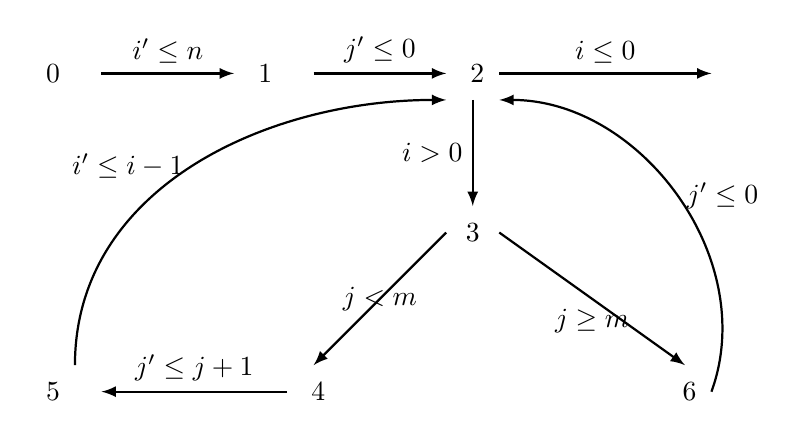
\begin{tikzpicture}[scale=\textwidth/18cm,samples=200]
\draw[] (-8, 10) circle (0pt) node{{ $0$}};
\draw[] (-4, 10) circle (0pt) node{{ $1$}};
\draw[] (0, 10) circle (0pt) node{{ $2$}};
\draw[] (0, 7) circle (0pt) node{{$3$}};
\draw[] (-3, 4) circle (0pt) node{{ $4$}};
\draw[] (-8, 4) circle (0pt) node{{ $5$}};
\draw[] (4, 4) circle (0pt) node{{ $6$}};
\draw[] (5, 10) circle (0pt) node {\textbf{$\lex$}};
%
\draw[ thick, -latex] (-7, 10)  -- node [above] {$i' \leq n$}(-4.5, 10);
\draw[ thick, -latex] (-3, 10)  -- node [above] {$j' \leq 0$}(-0.5, 10);
\draw[ thick, -latex] (0, 9.5)  -- node [left] {$i > 0$} (0, 7.5) ;
\draw[ thick, -latex] (0.5, 7)  -- node [below] {$ j \geq m $}  (4, 4.5);
\draw[ thick, -latex] (-7.5, 4.5)  to  [out=90,in=180]  node [left] {$i' \leq i - 1$ }(-0.5, 9.5);
\draw[ thick, -latex] (4.5, 4)  to  [out=70,in=0]   node [right] {$j' \leq 0 $}(0.5, 9.5);
\draw[ thick, -latex]  (-0.5, 7) -- node  {$j < m$}  (-3, 4.5) ;
\draw[ thick, -latex]  (-3.5, 4) -- node [above] {$j' \leq j + 1$}  (-7, 4) ;
\draw[ thick, -latex] (0.5, 10)  -- node [above] {$i \leq 0$}  (4.5, 10);
\end{tikzpicture}
    \caption{}
\end{centering}
\end{subfigure}
{
\begin{subfigure}{.95\textwidth}
\begin{centering}
    $\tpath_0 = 0 \to 1 \to 2$,
    $\tpath_2 = 2 \to 3 \to 6 \to 2$, 
    $\tpath_1 = 2 \to 3 \to 4 \to 5 \to 2$,
    $\tpath_3 = 2 \to \lex$
    \caption{}
\end{centering}
\end{subfigure}
}
{
\begin{subfigure}{.4\textwidth}
\begin{centering}
$
\tpath_0; 
\rpchoose{ 2: \tpath_1, 2: \tpath_2 }; \tpath_3.
$
\caption{}
\end{centering}
\end{subfigure}
}
\begin{subfigure}{.5\textwidth}
  \begin{centering}
  $
  \tpath_0 ; 
  \rpchoose{2: \rprepeat(\rprepeat(\tpath_1); \tpath_2), 
  2: \rprepeat(\tpath_1)}; \tpath_3.
  $
  \caption{}
\end{centering}
  \end{subfigure}
  \vspace{-0.4cm}
\caption{
(a) The two paths loop example.
(b) The abstract transition graph for $\kw{twoPathsWhile}(n, m)$.
(c) The simple transition paths.
(d) The rewrote program.
(e) The refined program.}
    \label{fig:whileTwoCounters-refine}
\end{figure}
}

To know the bounds for locations on different branches of a loop, 
it is necessary to know the execution orders of the two paths.

Over its abstract transition graph in Figure~\ref{fig:whileTwoCounters-refine}(b), we first collect all its simple transition path as in Figure~\ref{fig:whileTwoCounters-refine}(c).
Then we transform the multiple-path loop by computing the interleaving between paths explicitly and
generates a refined program $\rprog$ as the bottom part of Figure~\ref{fig:whileTwoCounters-refine}.

We first compute that $\tpath_1$ can iterate on itself, so there is one possible execution sub-order,
$\rprepeat(\tpath_1)$.
We recursively compute that after $\tpath_1$ done with the iteration on itself,
either the iteration of the original loop is finished
or $\tpath_2$ can execute right after.
For the first case, we compute a complete execution order $\rprepeat(\tpath_1)$.
In the second case, we again have a possible execution sub-order, $\rprepeat(\tpath_1); \tpath_2$.
After execution of $\tpath_2$, we compute that $\tpath_1$ iterates on itself again
and goes back to the same execution sub-order. 
The refinement algorithm finds this repetition and generate a complete execution order
$\rprepeat(\rprepeat(\tpath_1); \tpath_2)$.
Then the algorithm finish the refinement process since all the paths are visited and there is no more sub-orders. 
%  In the first one, $\tpath_2$ will be executed after all the iterations of $\tpath_1$ are done, and in the second one,
%  the entire loop is done after $\tpath_1$ finishes the iteration.
The refined program then is constructed below as in Figure~\ref{fig:whileTwoCounters-refine}(e).
\[
   \tpath_0 ; 
   \rpchoose{2: \rprepeat(\rprepeat(\tpath_1); \tpath_2), 
   2: \rprepeat(\tpath_1)}; \tpath_3.
\]

From this refined program, we can explicitly tell two possible path interleaving patterns.
With the explicit interleaving patterns, the following computation based on this refined program can compute more accurate reachability-bounds.
